\section{Requirements Engineering}
\subsection{The CaSh Case Study}
\begin{figure}[h]
    \centering
    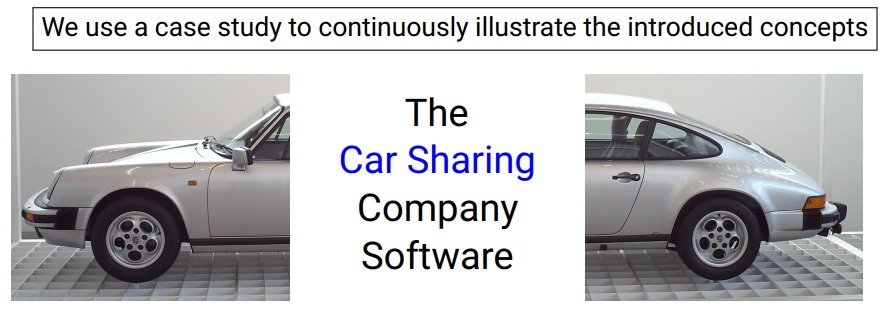
\includegraphics[width=1\textwidth]{Images/The CaSh Case Study.jpeg}
\end{figure}

\subsubsection*{Description}
\begin{defBox}[title=Main Roles \& Functionalities]
	\begin{itemize}
		\item Role-independent
		\begin{itemize}
			\item Authentication
		\end{itemize}
		\item Administrator
		\begin{itemize}
			\item Add/change new cars, rental locations
			\item Billing
		\end{itemize}
		\item User
		\begin{itemize}
			\item Check availability
			\item Request booking
			\item Change booking
		\end{itemize}
		\item Service Staff
		\begin{itemize}
			\item Take out vehicle for service 
		\end{itemize}
	\end{itemize}
\end{defBox}

\clearpage
\subsubsection*{Provision of services for different actors}
\begin{figure}[h]
    \centering
    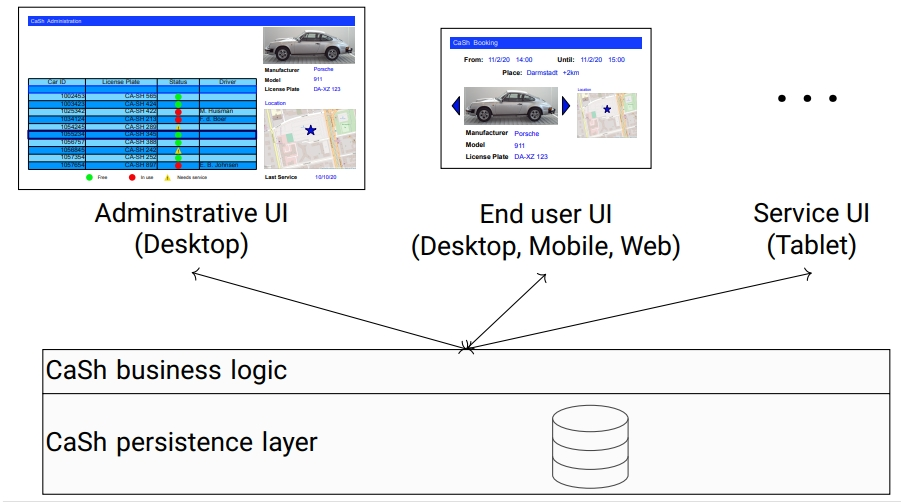
\includegraphics[width=0.87\textwidth]{Images/Provision of services for different actors.jpeg}
\end{figure}

\subsubsection*{Requirements Engineering}
\begin{figure}[h]
    \centering
    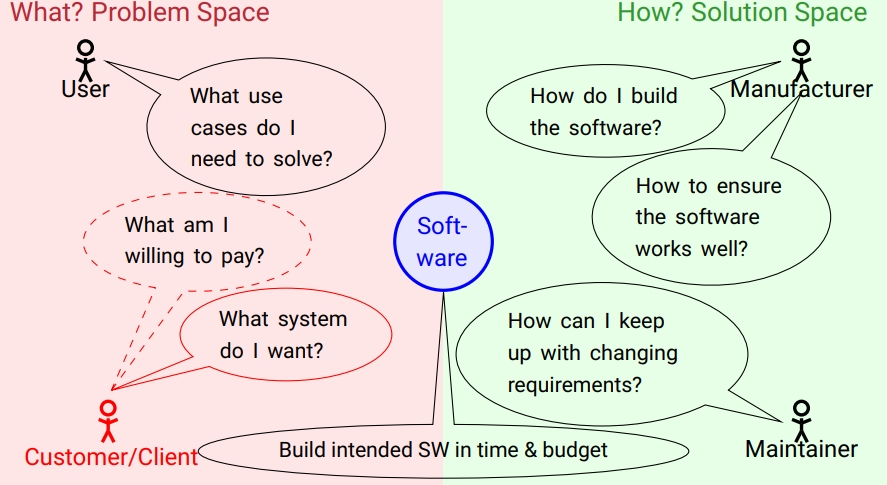
\includegraphics[width=0.87\textwidth]{Images/Requirements Engineering.jpeg}
\end{figure}

\clearpage
\subsection*{Requirements Engineering}
\blue{Assume:} You are contracted by \red{client} to develop CaSh
\begin{defBox}
	Systematic approach to the question: \red{What} has to be developed?
\end{defBox}
\begin{itemize}
	\item Understanding the problems in requirements elicitation 
	\item Different kinds of requirements
	\item Requirement engineering workflow
	\item Modelling requirements (next lecture)
	\begin{itemize}
		\item Scenarios \& Use cases
		\item Notations: Textual \& Graphical
	\end{itemize}
\end{itemize}

\subsection{Why Requirements Analysis is Difficult}
Mary had a little lamb.\\
What does the sentence mean?
\begin{defBox}[title=Meanings of to have]
	\begin{enumerate}
		\item to hold in possession as a property
		\item to trick or fool someone (been had by a someone)
		\item to beget or bear (habe a baby)
		\item to partake (have as a meal)
		\item ...
	\end{enumerate}
\end{defBox}
\begin{defBox}[title=Meanings of lamb]
	\begin{enumerate}
		\item a young sheep less than one year
		\item the young of various other animals (antelope, etc.)
		\item a person as gentle or weak as a lamb
		\item a person easily cheated or deceived
		\item the flesh of lamb used as food
		\item ...
	\end{enumerate}
\end{defBox}
Mary hd a little lamb\\
What does the sentence mean?
\blue{Possible Meanings:}
\begin{itemize}
	\item Mary owned once a lamb under one year
	\item Mary gave birth to an antelope
	\item ...
\end{itemize}
\begin{infoBox}
    Zusammengefasst verdeutlicht diese Beispiele, dass Sprache oft mehrdeutig ist, und genau diese Mehrdeutigkeit macht es im Requirements Engineering schwer, präzise Anforderungen zu spezifizieren.
\end{infoBox}

\subsection*{Application to Case Study?}
\begin{defBox}[title=What is meant with ...?] 
	\begin{itemize}
		\item \enquote{The status of a car is \red{in use}, \red{free} or \red{need service}.}
		\item \enquote{Each car must have a unique license plate number.}\\
		What if the care has not yet been registered?
		\item \enquote{Das System muss sicher sein.}\\
		\enquote{\red{sicher}} in welchem Sinne? secure or safe?
		\item Exercise: find ambiguous specifications in an API of your choice
	\end{itemize}
\end{defBox}

\subsection{What are Requirements?}
\begin{defBox}[title=Definition(Requirements)]
	Requirements are the descriptions of 
	\begin{itemize}
		\item the \red{services provided by the system} and
        \begin{infoBox}
            Den Dienstleistungen oder Funktionen, die das System bereitstellen soll.
            \begin{itemize}
                \item Zum Beispiel: Ein Online-Shop sollte es Benutzern ermöglichen, Produkte zu suchen, in den Warenkorb zu legen und zu bezahlen.
            \end{itemize}
        \end{infoBox}
		\item the \red{operational constraints}
        \begin{infoBox}
            Den betrieblichen Einschränkungen oder Rahmenbedingungen, unter denen das System arbeitet
            \begin{itemize}
                \item Zum Beispiel: Das System muss mindestens 100 Datenbankabfragen pro Sekunde verarbeiten können (Datenbank-Durchsatz).
                \item Weitere Beispiele sind Anforderungen an den Speicherbedarf des Systems oder an unterstützte Navigationssysteme (z.B. GPS, Galileo, GLONASS).
            \end{itemize}
        \end{infoBox}
	\end{itemize}
\end{defBox}
\begin{defBox}
	\begin{itemize}
		\item Database throughput (number of database queries per second)
		\item System memory
		\item Navigation systems GPS, Galileo, GLONASS
		\item ...
	\end{itemize}
\end{defBox}

\clearpage
Requirements are written down
\begin{itemize}
	\item in the \red{System Requirements Specification} (SRS) Document (German: Pflichtenheft)
	\item as \red{user stories}, structured natural language, use cases, state diagrams, ... and stored in the \red{product backlog} (ordered list of requirements)
\end{itemize}
\begin{infoBox}
    \fatsf{Wie werden Anforderungen dokumentiert?}\\
    \begin{enumerate}
        \item \fatsf{System Requirements Specification (SRS)}, auf Deutsch oft als \fatsf{Pflichtenheft} bezeichnet.
        \begin{itemize}
            \item Das SRS ist ein strukruriertes Dokument, das alle Anforderungen an das System detailliert beschreibt.
            \item Es ist die Grundlage für die Entwicklung und dient als Referenz für die Überprüfung, ob die Anforderungen erfüllt wurden
        \end{itemize}
        \item \fatsf{Andere Darstellungsformen von Anforderungen:}
        \begin{itemize}
            \item \fatsf{User Stories:} Kurze, informelle Beschreibungen aus der Perspektive eines Benutzers. Beispiel: \enquote{Als Benutzer möchte ich nach Produkten suchen können, um das passende Angebot zu finden.}
            \item \fatsf{Strukturiertes natürliches Englisch:} Eine präzise, aber leicht verständliche Form der Beschreibung.
            \item \fatsf{Use Cases:} Szenarien, die beschreiben, wie Bunutzer das System in verschiedenen Situationen nutzen.
            \item \fatsf{Zustandsdigramme:} Grafische Darstellungen der Zustände eines Systems und deren Übergänge.
        \end{itemize}
        \item \fatsf{Product Backlog:} Eine geordnete Liste der Anforderungen.
        \begin{itemize}
            \item Im agilen Entwicklungsansatz (z.B. Scrum) werden Anforderungen im Product Backlog gesammelt und priorisiert.
            \item Das Backlog ist dynamisch, d.h., es wird im Laufe des Projekts immer wieder aktualisiert.
        \end{itemize}
    \end{enumerate}
\end{infoBox}
\begin{defBox}
	Requirements are \red{not} solutions
\end{defBox}
\begin{infoBox}
    \begin{itemize}
        \item Anforderungen beschreiben, \fatsf{was} das System tun soll oder \fatsf{unter welchen Bedingungen} es arbeiten soll, aber nicht \fatsf{wie} es das erreichen soll.
        \item z.B.: Eine Anforderung könnte sein, dass die Suchfunktion innerhalb von 2 Sekunden Ergebnisse liefern muss. Diese Anforderung sagt nichts darüber aus, wie diese Geschwindigkeit technisch erreicht wird.
    \end{itemize}
\end{infoBox}
\subsection{Requirement Types}
\begin{defBox}[title=Many Different Types of Requirements]
	\begin{itemize}
		\item \red{User} requirements
		\item \red{System} requirements
		\item \red{Functional} requirements
		\item \red{Non-functional} requirements
		\item \red{Domain} requirements
	\end{itemize}
	\blue{Let's discuss them in turn}
\end{defBox}
\subsubsection{User Requirements}
\begin{defBox}[title=User Requirements]
	State in natural language and (semi-formal) diagrams:
	\begin{itemize}
		\item What are the \red{services} expected to be provided by the system
		\item What are the \red{operational constraints} (Betriebsparameter)
	\end{itemize}
	Often high-level and abstract descriptions (normally \red{written by the customer})
\end{defBox}
\begin{infoBox}
    Benutzeranforderungen (User Requirements) sind Anforderungen, die aus der Perspektive der Benutzer oder Kunden beschrieben werden. Sie geben an, \fatsf{welche Dienste das System bereitstellen soll} und \fatsf{welche Betriebsparameter oder Einschränkungen} dabei gelten. Benutzeranforderungen sind oft \fatsf{hochgradig, abstrakt und allgemein formuliert}, um die grundlegenden Erwartungen an das System auszudrücken. Normalerweise werden sie vom Kunden oder den Stakeholdern verfasst.\\
    \fatsf{Merkmale von Benutzeranforderungen:}
    \begin{enumerate}
        \item \fatsf{Formulierung in natürlicher Sprache und Diagrammen:}
        \begin{itemize}
            \item Benutzeranforderungen werden oft in \fatsf{natürlicher Sprache} beschrieben, damit sie für alle Beteiligten (einschließlich Kunden und Entwickler) verständlich sind.
            \item \fatsf{Semi-formale Diagramme} wie Use-Case-Diagramme oder einfache Ablaufdiagramme können verwendet werden, um die Anforderungen graphisch darzustellen und besser zu veranschaulichen.
        \end{itemize}
        \item \fatsf{Beschreiben der erwarteten Dienste des Systems:}
        \begin{itemize}
            \item Es wird festgelegt, \fatsf{welche Funktionalitäten} oder \fatsf{Dienste} das System bereitstellen soll, ohne dabei zu sehr ins Detail zu gehen, wie diese technisch umgesetzt werden.
            \item Beispiel: \enquote{Das System soll es Benutzern ermöglichen, Flugtickets online zu buchen.}
        \end{itemize}
        \item \fatsf{Definieren von Betriebsparametern (operational contraints)}
        \begin{itemize}
            \item Benutzeranforderungen enthalten auch \fatsf{Rahmenbedingungen}, unter denen das System funktionieren soll, z.B. gesetzliche Vorgaben, Leistungsanforderungen oder bestimmte Betriebsumgebungen.
            \item Beispiel: \enquote{Das System muss den deutschen Datenschutzbestimmungen entsprechen}
        \end{itemize}
    \end{enumerate}
\end{infoBox}
\begin{defBox}[title=Example]
	\enquote{CaSh shall keep track of all bookings as required by German law} (e.g., in case of speeding tickets, for tax purposes)
\end{defBox}
\begin{infoBox}
    \fatsf{CaSh soll alle Buchungen gemäß den Anforderungen des deutschen Rechts nachverfolgen (z.B. Geschwindigkeitsverstöße oder steuerliche Zwecke)}\\
    Die Anforderung drückt aus, dass das System \fatsf{alle Buchungen aufzeichnen und verwalten soll}, um den gesetzlichen Anforderungen gerecht zu werden. Es wird jedoch \fatsf{nicht spezifiziert}, wie das System dies technisch tun soll oder welche Datenbanktechnologien verwendet werden sollen. Es bleibt auf einer \fatsf{hohen, abstrakten Ebene.}
\end{infoBox}

\clearpage
\subsubsection{System Requirements}
\begin{defBox}[title=System Requirements (Systemanforderungen)]
	\red{Precise and detailed} specification of the system's
	\begin{itemize}
		\item functions, services and
		\item operational constraints
	\end{itemize}
\end{defBox}
\begin{infoBox}
    Systemanforderungen (System Requirements) sind \fatsf{präzise und detaillierte Spezifikationen} darüber, was ein System leisten soll. Sie bauen auf den Benutzeranforderungen auf, sind jedoch genauer und technischer. Systemanforderungen legen fest, \fatsf{welche Funktionen und Dienstleistungen} das System bereitstellen muss und \fatsf{unter welchen Betriebsbedingungen} es funktionieren soll.
\end{infoBox}
\begin{defBox}[title=Example (CaSh System Requirements)]
    \begin{itemize}
        \item \enquote{Upon successful completion of a booking, the user must be shown an overview of the booking details.}
        \item \enquote{Booking details must be stored by CaSh for 10 years from the booking date onwards.}
        \item \enquote{Booking details consist of pickup and return date, care details (license plate number, ...), user name + address and payment information.}
    \end{itemize}
\end{defBox}
\begin{infoBox}
    \begin{enumerate}
        \item \enquote{Nach erfolgreichem Abschluss einer Buchung muss dem Benutzer eine Übersicht der Buchungsdetails angezeigt werden.}
        \item \enquote{Buchungsdetails müssen von CaSh für 10 Jahre ab dem Buchungsdatum gespeichert werden.}
        \item \enquote{Buchungsdetails bestehen aus Abhol- und Rückgabedatum, Fahrzeugdetails (z.B. Kennzeichnen), Benutzername, Adresse und Zahlungsinformationen.}
    \end{enumerate}
\end{infoBox}

\clearpage
\begin{defBox}[title=Characteristics of system requirements:]
    \begin{itemize}
        \item \red{Refinement} of user requirements
        \item Determine the \red{system interface} (functional, \red{not} technical interface) $\implies$ Define \red{solution space}
        \item Recorded as part of the \red{system requirements document} (functional specification) and typically part of the contract with client
        \item Authored by \red{software developer} or \red{business analyst} in collaboration with \red{client}
        \item (Dt.: Grundlage für das Pflichtenheft)
    \end{itemize}
\end{defBox}
\begin{infoBox}
    \fatsf{Merkmale der Systemanforderungen:}
    \begin{enumerate}
        \item \fatsf{Verfeinerung der Benutzeranforderungen}
        \begin{itemize}
            \item Während Benutzeranforderungen \fatsf{allgemein} formuliert sind, werden sie durch die Systemanforderungen in \fatsf{spezifische und messbare Anforderungen} übersetzt.
            \item Sie konkretisieren, \fatsf{wie die in den Benutzeranforderungen beschriebenen Erwartungen erfüllt werden sollen.}
        \end{itemize}
        \item \fatsf{Definition der Systemschnittstellen:}
        \begin{itemize}
            \item Systemanforderungen legen fest, \fatsf{wie das System mit anderen Systemen, Benutzern oder Geräten interagiert,} ohne jedoch die genauen technischen Implementierungsdetails anzugeben.
            \item Es wird der \fatsf{Lösungsraum} definiert, d.h., welche Ansätze oder Technologien zur Erfüllung der Anforderungen verwendet werden können
        \end{itemize}
        \item \fatsf{Teil der Systemanforderungsdokumentation:}
        \begin{itemize}
            \item Die Anforderungen werden im \fatsf{System Requirements Specification (SRS)} festgehalten, das häufig auch als \fatsf{Pflichtenheft} bezeichnet wird.
            \item Das SRS-Dokument ist oft ein \fatsf{Bestandteil des Vertrags} zwischen dem Kunden und dem Entwickler, da es genau beschreibt, was geliefert werden muss.
        \end{itemize}
        \item \fatsf{Erarbeitet durch Entwickler oder Business Analysten in Zusammenarbeit mit dem Kunden:}
        \begin{itemize}
            \item Systemanforderungen werden typischerweise von \fatsf{Softwareentwicklern oder Business-Analysten} verfasst, die eng mit dem Kunden zusammenarbeiten, um sicherzustellen, dass die Spezifikationen den Anforderungen und Erwartungen entsprechen.
        \end{itemize}
    \end{enumerate}
\end{infoBox}
\subsubsection{Functional Requirements}
\begin{defBox}[title=Functional requirement ($\neq$ functional specification)]
    Functionality that is clearly identifiable and localized in the \red{code}
\end{defBox}
\begin{infoBox}
    Funktionale Anforderungen sind spezifische Beschreibungen von \fatsf{Funktionen oder Dienstleistungen,} die ein System bereitstellen soll. Sie geben an, \fatsf{was das System tun soll,} ohne dabei zu beschreiben, \fatsf{wie} es technisch umgesetzt wird. Funktionale Anforderungen sind \fatsf{direkt im Code nachvollziehbar}, da sie sich auf klare definierte Funktionen beziehen, die im System implementiert werden.
\end{infoBox}
\begin{defBox}[title=Functional Requirements Specify ...]
    \begin{itemize}
        \item Services to be provided by the system, for instance:
        \begin{itemize}
            \item Authentication
            \item Querying for available cars
            \item Sending confirmation emails
        \end{itemize}
        \item \red{System reactions} to specific inputs/events, for instance:
        \begin{itemize}
            \item Error message when selected return date is before pick up date
        \end{itemize}
        \item \red{System behavior} in specific situations, for instance:
        \begin{itemize}
            \item Network disruption during booking process
        \end{itemize}
    \end{itemize}
\end{defBox}
\begin{infoBox}[title=Was spezifizieren funktionale Anforderungen]
    Funktionale Anforderungen legen fest, welche \fatsf{Dienstleistungen, Systemreaktionen und Systemverhalten} in bestimmten Situationen das System bieten soll:
    \begin{enumerate}
        \item \fatsf{Dienste, die vom System bereitgestellt werden:}
        \begin{itemize}
            \item Diese Anforderungen beschreiben, \fatsf{welche spezifischen Funktionen das System bieten soll.}
            \item Beispiele:
            \begin{itemize}
                \item \fatsf{Authentifizierung:} Das System muss es Benutzern ermöglichen, sich mit Benutzernamen und Passwort anzumelden.
                \item \fatsf{Abfragen nach verfügbaren Autos}
                \item \fatsf{Versenden von Bestätigungs-E-Mails} 
            \end{itemize}
        \end{itemize}
        \item \fatsf{Systemreaktionen auf bestimmte Eingaben oder Ereignisse:}
        \begin{itemize}
            \item Funktionale Anforderungen geben an, \fatsf{wie das System auf bestimmte Benutzeraktionen oder Ereignisse reagieren soll.}
            \item Beispiel: \fatsf{Fehlermeldung bei ungültigen Eingaben:} Wenn das Rückgabedatum vor dem Abholdatum liegt, muss das System eine Fehlermeldung anzeigen.
        \end{itemize}
        \item \fatsf{Systemverhalten in spezifischen Situationen:}
        \begin{itemize}
            \item Sie spezifizieren, \fatsf{wie das System sich in bestimmten Ausnahmefällen oder besonderen Umständen verhalten soll.}
            \item Beispiel: \fatsf{Netzwerkunterbrechung während des Buchungsvorgangs:} Das System muss in der Lage sein, den Buchungsvorgang bei einer Netzwerkunterbrechung wiederaufzunehmen oder die Benutzer entsprechend zu informieren.
        \end{itemize}
    \end{enumerate}
\end{infoBox}
\begin{infoBox}[title=Unterschied zu einer funktionalen Spezifikationen]
    \begin{itemize}
        \item \fatsf{Funktionale Anforderungen} beschreiben \fatsf{was} das System leisten soll (z.B. bestimmte Funktionen, Dienste oder Reaktionen), während eine \fatsf{funktionale Spezifikation} detailliert beschreibt, \fatsf{wie} diese Anforderungen technisch umgesetzt werden sollen.
        \item Beispiel: Eine funktionale Anforderung könnte sein, dass Benutzer sich anmelden können, während die funktionale Spezifikation festlegt, welche Verschlüsselungsprotokolle und Sicherheitsmechanismen für die Anmeldung verwendet werden.
    \end{itemize}
\end{infoBox}
\subsubsection{Non-Functional Requirements}
\begin{defBox}[title=Non-functional Requirements (NFR)]
    Constraints on the services or functions offered by the system, including:
    \begin{itemize}
        \item Service level agreement (SLA)
        \item Constraints from development process (sequential/incremental)
        \item Alignment to standards (for example, protocols)
    \end{itemize}
\end{defBox}
\begin{infoBox}
    Nicht-funktionale Anforderungen (Non-functional Requirements, NFR) beschreiben \fatsf{Einschränkungen oder Rahmenbedingungen}, unter denen die Funktionen eines Systems bereitgestellt werden müssen. Sie betreffen die \fatsf{Qualitätsmerkmale} des Systems und beziehen sich auf \fatsf{Leistung, Sicherheit, Benutzerfreudlichkeit, Zuverlässigkeit} usw., anstatt auf spezifische Funktionen.
\end{infoBox}
\begin{defBox}
    NFRs are often cross-cutting concerns that apply to the whole system
\end{defBox}
Meeting such requirements is usually impossible by adding a piece of code at a specific location or cannot be guranteed by software alone.
\begin{infoBox}[title=Merkmale nicht-funktionaler Anforderungen]
    \begin{enumerate}
        \item \fatsf{Oft systemübergreifende Anforderungen:}
        \begin{itemize}
            \item Sie sind \fatsf{querschnittliche Anforderungen}, die für mehrere oder alle Teile des Systems gelten, wie z.B. Sicherheitsstandards oder Antwortzeiten.
        \end{itemize}
        \item \fatsf{Schwer durch einfache Code-Änderungen zu erfüllen:}
        \begin{itemize}
            \item Es ist oft \fatsf{nicht möglich, eine nicht-funktionale Anforderung durch Hinzufügen von Code an einer bestimmten Stelle zu erfüllen.} Sie erfordern meist \fatsf{übergreifende Maßnahmen im gesamten System.}
            \item Zum Beispiel ist es nicht genug, nur an einer Stelle im Code Änderungen vorzunehmen, um die \fatsf{Gesamtleistung oder Sicherheit} des Systems sicherzustellen.
        \end{itemize}
    \end{enumerate}
\end{infoBox}

\begin{defBox}[title=Example (CaSh non-functional requirements)]
    \begin{itemize}
        \item The database must be able to process 1000 queries (Abfragen) per second
        \begin{infoBox}
            Diese Anforderung betrifft die \fatsf{Leistungsfähigkeit} des Systems.
        \end{infoBox}
        \item User data must only be accessible to authorized persons
        \begin{infoBox}
            Diese Anforderung bezieht sich auf die \fatsf{Sicherheit und Datenschutz} im System.
        \end{infoBox}
        \item The software development model must be CMMI Level 4 certified
        \begin{infoBox}
            \textbf{Diese Anforderung beschreibt eine \fatsf{Prozessanforderung} und legt fest, welches Entwicklungsmodell verwendet werden soll.}
        \end{infoBox}
        \item CaSh must provide the booking data for the accounting system (Buchhaltungssystem)
        \begin{infoBox}
            Diese Anforderung betrifft die \fatsf{Interoperabilität}, also die Fähigkeit des Systems, mit anderen Systemen zusammenzuarbeiten.
        \end{infoBox}
    \end{itemize}
\end{defBox}

\clearpage
\begin{defBox}[title=Non-functional requirements]
    \begin{enumerate}
        \item \red{Product requirements}
        \begin{itemize}
            \item Reliability, availability
            \item Effeciency (performance, memory)
            \item Usability
            \item Portability
        \end{itemize}
        \item \red{Organisational requirements}
        \begin{itemize}
            \item Delivery mode (beta, continuous, ...)
            \item Implementation (programming language, frameworks, ...)
            \item Standardization (ISO 9000, CMMI, ...)
        \end{itemize}
        \item \red{External requirements}
        \begin{itemize}
            \item Interoperability (TUCaN-Moodle)
            \item Ethical aspects
            \item Legal aspects (safety, security, privacy, ...)
        \end{itemize}
    \end{enumerate}
\end{defBox}
\begin{infoBox}[title=Arten von nicht-funktionalen Anforderungen:]
    \begin{enumerate}
        \item \fatsf{Produktanforderungen:}
        \begin{itemize}
            \item Betreffen die \fatsf{Eigenschaften des Produkts}, wie \fatsf{Zuverlässigkeit, Verfügbarkeit, Effizienz, Benutzerfreundlichkeit und Portabilität.}
            \item Beispiel: \enquote{Die Software muss in weniger als 2 Sekunden auf eine Benutzeranfrage reagieren.}
        \end{itemize}
        \item \fatsf{Organisatorische Anforderungen:}
        \begin{itemize}
            \item Beziehen sich auf \fatsf{organisatorische Rahmenbedingungen}, wie \fatsf{Liefermode, Entwicklungsprozesse, Standards und Zertifizierungen}
            \item Beispiel: \enquote{Die Software muss nach ISO 9000 zuertifiziert sein.}
        \end{itemize}
        \item \fatsf{Externe Anforderungen:}
        \begin{itemize}
            \item Beziehen sich auf \fatsf{gesetzliche, ethische oder externe technische Anforderungen}, wie \fatsf{Datenschutzgesetze, Sicherheitsvorschriften oder Interoperabilität mit anderen Systemen.}
            \item Beispiel: \enquote{Die Software muss die Datenschutz-Grundverordnung (DSGVO) einhalten.}
        \end{itemize}
    \end{enumerate}
\end{infoBox}

\clearpage
\subsubsection{Functional vs. Non-Functional Requirements}
\begin{defBox}[title=Observations]
    Non-functional requirements ...
    \begin{itemize}
        \item may result in the identification of functional requirements
        \item are often more mission-critical than individual functional requirements
    \end{itemize}
\end{defBox}
\begin{defBox}[title=Example (Relative importance of non-functional requirements)]
    A car shring system that does not support to confirm a booking by email is still usable; if the system is not secure or reliable, it is worthless.
\end{defBox}
\begin{infoBox}[title=Beobachtungen zum Unterschied:]
    \begin{itemize}
        \item \fatsf{Nicht-funktionale Anforderungen können funktionale Anforderungen identifizieren:}
        \begin{itemize}
            \item Wenn zum Beispiel eine nicht-funktionale Anforderung lautet, dass das System \fatsf{sicher sein muss}, kann daraus eine funktionale Anforderung entstehen, wie das \fatsf{Implementieren von Benutzerzugriffsrechten oder einer Zwei-Faktor-Authentifizierung.}
            
        \end{itemize}
        \item \fatsf{Nicht-funktionale Anforderungen sind oft kritischer für das Gesamtsystem:}
        \begin{itemize}
            \item Während ein System möglicherweise ohne bestimmte \fatsf{funktionale Anforderungen} noch funktionieren kann (z.B. das Versenden von E-Mails), könnte es \fatsf{unbrauchbar sein}, wenn es die \fatsf{nicht-funktionalen Anforderungen} wie \fatsf{Sicherheit, Zuverlässigkeit oder Leistung} nicht erfüllt.
            \item \fatsf{Beispiel:} Ein Carshring-System, das keine Buchungsbestätigung per E-Mail senden kann, ist immer noch nutzbar. Wenn das System jedoch \fatsf{unsicher oder unzuverlässig} ist, verliert es seinen Wert, da Benutzer ihm nicht vertrauen würden und es nicht zuverlässig genutzt werden kann.
        \end{itemize}
    \end{itemize}
\end{infoBox}

\subsubsection{Ensuring Verifiability of Non-Functional Requirements}
How to ckeck whether non-functional requirements are met?
\begin{defBox}[title=Example (Typical usability requirement)]
    \enquote{The user interface should be easy to use.}
\end{defBox}
\begin{defBox}[title=Problems with this Requirement]
    \begin{itemize}
        \item How to measure \enquote{easy}?
        \item Easy for \red{whom}?
        \begin{itemize}
            \item Expert user
            \item Average user
            \item Persons with a handicap (accessiblity)
        \end{itemize}
    \end{itemize}
\end{defBox}
\begin{infoBox}
    \fatsf{\enquote{Die Benutzeroberfläche sollte leicht zu bedienen sein.}} Diese Anforderung ist subjektiv und schwer messbar. Daher wird sie in konkrete Anforderungen umgewandelt:
\end{infoBox}
\begin{defBox}[title=Concretise Formulation into Quantifiable Requirements]
    \begin{itemize}
        \item \enquote{\red{Agents} can assist in bookings and manage the car pool after one day of training}
        \item \enquote{An average \red{end user} can complete a booking in less than 5 minutes}
        \item \enquote{The user interface has scalable fonts and pop-up help text}
    \end{itemize}
\end{defBox}

\subsubsection{Domain Requirements}
\begin{infoBox}
    Domänenanforderungen sind Anforderungen, die aus der \fatsf{spezifischen Anwendungsdomäne} eines Systems abgeleitet werden, anstatt direkt aus den Bedürfnissen der Benutzer. Sie beziehen sich auf \fatsf{Regeln, Vorschriften, Standards oder Prozesse}, die für eine bestimmte Branche oder Anwendung typisch sind.
\end{infoBox}
\begin{defBox}[title=Domain Requirements]
    Derived from \red{application domain} rather than from the needs of the needs of the user
    \begin{itemize}
        \item Expressed in \red{damain-specific language} and hard to understand by software engineers
        \item Often \red{implicitly assumed} as obvious to domain experts
        \item Functional or non-functional
    \end{itemize}
\end{defBox}
\begin{defBox}[title=Example]
    Car sharing companies are required to check that new customers have a driving licence.
\end{defBox}
\begin{infoBox}[title=Merkmale von Domänenanforderungen:]
    \begin{enumerate}
        \item \fatsf{Ausgedrückt in domänenspezifischer Sprache:}
        \begin{itemize}
            \item Domänenanforderungen werden häufig in einer Sprache formuliert, die \fatsf{für Domänenexperten verständlich} ist, aber \fatsf{für Softwareingenieure schwer zu verstehen} sein kann.
            \item Das bedeutet, dass sie \fatsf{technische Begriffe oder Fachjargon} aus der betreffenden Branche enthlaten können.
        \end{itemize}
        \item \fatsf{Häufig als selbstverständlich vorausgesetzt:}
        \begin{itemize}
            \item Domänenexperten nehmen oft an, dass diese Anforderungen \fatsf{offensichtlich} und für jeden verständlich sind, was dazu führen kann, dass sie \fatsf{nicht explizit dokumentiert} werden.
            \item Dies kann zu \fatsf{Missverständnisse oder fehlenden Anforderungen} führen, wenn sie nicht korrekt an das Softwareentwicklungsteam kommuniziert werden.
        \end{itemize}
        \item \fatsf{Können funktional oder nicht-funktional sein:}
        \begin{itemize}
            \item \fatsf{Funktionale Domänenanforderungen} beziehen sich auf bestimmte Funktionen, die das System ausführen muss, um den Anforderungen der Domäne zu entsprechen.
            \item \fatsf{Nicht-Funktionale Domänenanforderungen} können Einschränkungen oder Qualitätsmerkmale betreffen, die für die Domäne wichtig sind.
        \end{itemize}
    \end{enumerate}
\end{infoBox}
\begin{infoBox}[title=Warum sind Domänenanforderungen wichtig?]
    \begin{itemize}
        \item \fatsf{Domänenanforderungen stellen sicher, dass das System den spezifischen Anforderungen der Branche entspricht}, einschließlich rechtlicher, geschäftlicher und technischer Standards.
        \item Wenn Domänenanforderungen \fatsf{nicht korrekt erfasst oder verstanden} werden, kann es zu \fatsf{schwerwiegenden Problemen} kommen, z.B. dass das System \fatsf{gesetzliche Vorschriften nicht erfüllt.}
    \end{itemize}
\end{infoBox}

\subsubsection*{How to come Up with Requirements? Requirements Engineering Process}
\begin{defBox}[title=Requirements Engineering (RE)]
    Requirements engineering is the process of
    \begin{itemize}
        \item finding,
        \item analyzing,
        \item documenting, and
        \item validating
    \end{itemize}
    software requirements
\end{defBox}
The \red{system requirements document} is created and maintained during RE

\subsection{Requirements Engineering Process-Flow}
\begin{figure}[h]
    \centering
    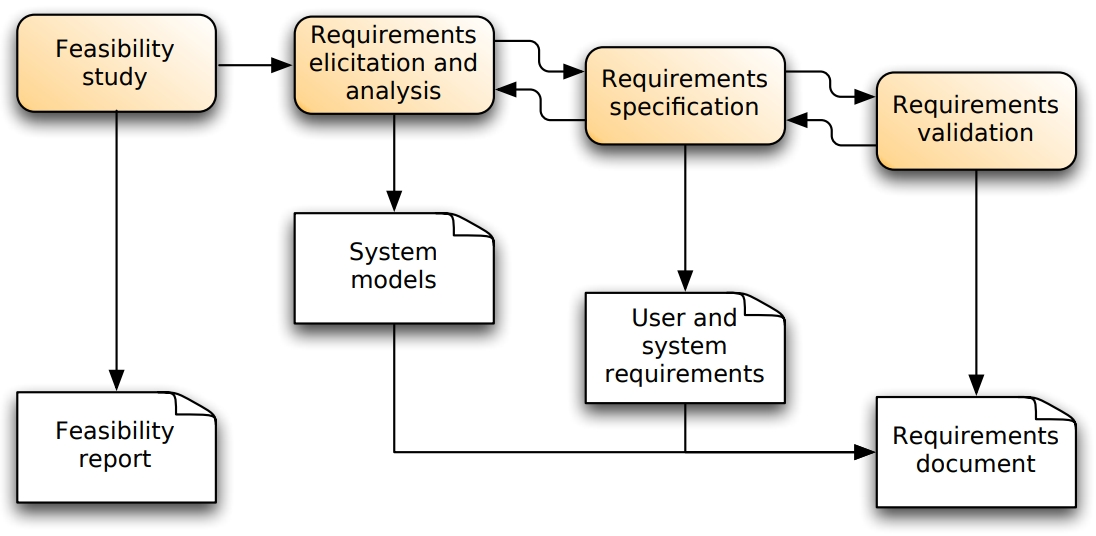
\includegraphics[width=1\textwidth]{Images/Requirements Engineering Process.jpeg}
\end{figure}

\clearpage
\subsection{RE Process}
\subsubsection*{Feasibility Study (Machbarkeitsstudie)}
\begin{infoBox}
    Die \fatsf{Machbarkeitsstudie} ist ein wichtiger Schritt im \fatsf{Requirements Engineering (RE)-Prozess} und dient dazu, eine fundierte Entscheidung darüber zu treffen, ob der \fatsf{Systementwicklungsprozess} begonnen oder fortgesetzt werden sollte. Sie hilft dabei, \fatsf{potenzielle Risiken und Herausforderungen} frühzeitig zu erkennen und abzuwägen, ob es sinnvoll ist, ein Projekt weiterzuverfolgen.
\end{infoBox}
\begin{defBox}[title=Objective of the Feasibility Study]
    Obtain a justified recommendation whether the requirements engineering and system development process should be \red{started} (or continued) based on:
    \begin{itemize}
        \item Preliminary business requirements (Vorläufige Geschäftsanforderungen)
        \begin{infoBox}
            Beschreibt die übergeordneten Ziele und Erwartungen, die das system erfüllen soll.
        \end{infoBox}
        \item Outline description of the system (Übersichtsbeschreibung des Systems)
        \begin{infoBox}
            Eine allgemeine Darstellung, wie das System funktionieren soll und welche Hauptfunktionen es bietet.
        \end{infoBox}
        \item Description of how the system is intended to support business processes (Beschreibung der Unterstützung von Geschäftsprozessen)
        \begin{infoBox}
            Erklärt, wie das System die Geschäftsprozesse des Unternehmens verbessern oder unterstützen wird.
        \end{infoBox}
    \end{itemize}
\end{defBox}
\begin{defBox}[title=Feasibility Report]
    \begin{itemize}
        \item Does the system contribute to the \red{overall objectives} of the organization?
        \item Can the system be \red{implemented} uing current technology and within given cost and schedule constraints?
        \item Can the system be \red{integrated} with other systems used by the company?
    \end{itemize}
\end{defBox}

\begin{infoBox}[title=Ziele der Machbarkeitsstudie:]
    \begin{enumerate}
        \item \fatsf{Beurteilung, ob das geplante System die Geschäftsziele unterstützt:}
        \begin{itemize}
            \item Es wird untersucht, ob das System einen \fatsf{Mehrwert für die Organisation} schafft und zur \fatsf{Erreichung der Unternehmensziele} beiträgt.
        \end{itemize}
        \item \fatsf{Überprüfung der technischen Machbarkeit:}
        \begin{itemize}
            \item Es wird geprüft, ob das System mit der \fatsf{aktuellen Technologie} realisierbar ist. Es muss also festgestellt werden, ob die \fatsf{notwendigen technischen Ressourcen und Fähigkeiten} vorhanden sind, um das Projekt erfolgreich umzusetzen.
        \end{itemize}
        \item \fatsf{Bewertung von Kosten und Zeitrahmen:}
        \begin{itemize}
            \item Es wird analysiert, ob das System innerhalb der \fatsf{vorgegebenen Budget-und Zeitrahmen} realisierbar ist, um sicherzustellen, dass das Projekt wirtschaftlich sinnvoll ist.
        \end{itemize}
        \item \fatsf{Prüfung der Intergrationsfähigkeit mit anderen Systemen:}
        \begin{itemize}
            \item Es wird untersucht, ob das geplante System sich nahtlos in die \fatsf{bestehende IT-Landschaft} und die \fatsf{anderen Systeme des Unternehmens} intergrieren lässt.
        \end{itemize}
    \end{enumerate}
\end{infoBox}

\subsubsection*{Requirements Elicitation and Analysis}
\begin{infoBox}
    Der \fatsf{Requirements Elicitation and Analysis-Prozess} ist ein wichtiger Schritt im Requirements Engineering, bei dem es darum geht, \fatsf{systematisch die Anforderungen zu entdecken und zu analysieren}, die an das zu entwickelnde System gestellt werden. Ein effektiver Ansatz zur Anforderungsfindung ist der \fatsf{Viewpoint-orientierte Ansatz}, bei dem Anforderungen aus verschiedenen Perspektiven gesammelt und bewertet werden.
\end{infoBox}
\begin{figure}[h]
    \centering
    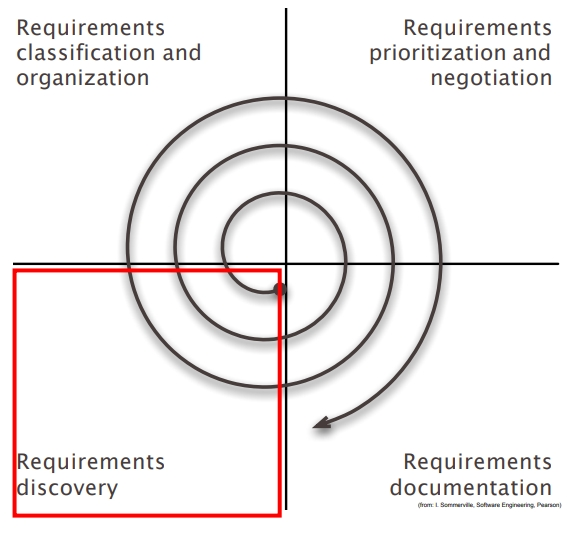
\includegraphics[width=0.5\textwidth]{Images/Requirements Elicitation and Analysis.jpeg}
\end{figure}
\begin{infoBox}[title=Viewpoint-orientierter Ansatz]
    Der \fatsf{Viewpoint-orientierte Ansatz} betrachtet die Anforderungen aus verschiedenen \fatsf{Blickwinkeln (Viewpoints)}, um sicherzustellen, dass alle relevanten Perspektiven abgedeckt sind. Dadurch wird das Risiko verringert, wichtige Anforderungen zu übersehen.
\end{infoBox}
\begin{defBox}[title=Systematic requirement descovery: Viewpoint-oriented Approach]
    \blue{Generic types of viewpoints}
    \begin{itemize}
        \item \red{Interactor} viewpoints: Persons (or systems) that will directly interact with the system such as end users, administrative \& servise personal \red{-direct stakeholders-}
        \item \red{Indirect} viewpoints: Stakeholders that influence the requirements, but who will not directly use the system, e.g. CFO (finances), data protection official \red{-indirect stakeholders-}
        \item \red{Domain} viewpoints: Domain characteristics \& constraints that influence the system requirements E.g., legal regulations on booking details and storage duration
    \end{itemize}
\end{defBox}
\begin{figure}
    \centering
    \begin{minipage}{0.3\textwidth}
        \centering
        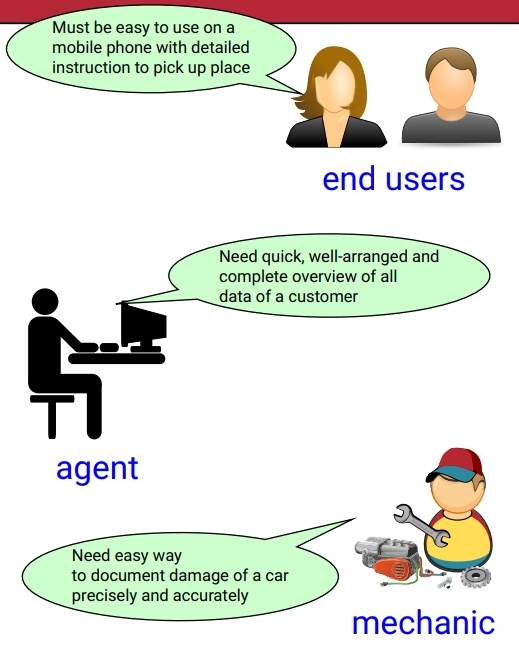
\includegraphics[width=\textwidth]{Images/Interactor viewpoints.jpeg}
        \caption{Interactor viewpoints}
    \end{minipage}\hfill
    \begin{minipage}{0.3\textwidth}
        \centering
        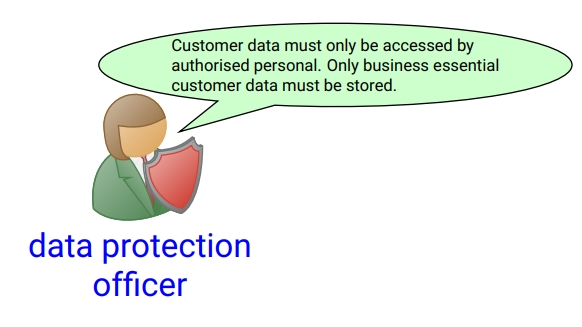
\includegraphics[width=\textwidth]{Images/Indirect viewpoints.jpeg}
        \caption{Indirect viewpoints}
    \end{minipage}\hfill
    \begin{minipage}{0.3\textwidth}
        \centering
        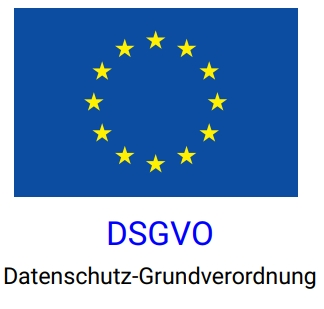
\includegraphics[width=\textwidth]{Images/Domain viewpoints.jpeg}
        \caption{Domain viewpoints}
    \end{minipage}
\end{figure}
\begin{defBox}[title=Systematic requirement discovery: Viewpoint-oriented Approach]
    \begin{itemize}
        \item Develop more specific viewpoints during elicitation
        \begin{infoBox}
            \begin{itemize}
                \item Während der Anforderungsanalyse können neue, spezifischere Viewpoints identifiziert werden, die zunächst vielleicht nicht offensichtlich waren.
                \item Beispielsweise könnten im Laufe der Analyse weitere Stakeholdergruppen oder spezielle technische Anforderungen entdeckt werden, die vorher nicht berücksichtigt wurden.
                \item Das hilft, detaillierte Anforderungen zu erfassen, die sonst möglicherweise übersehen worden wären.
            \end{itemize}
        \end{infoBox}
        \item Use most important viewpoints to discover requirements
        \begin{infoBox}
            \begin{itemize}
                \item Nicht alle Viewpoints sind gleich wichtig, daher konzentriert man sich zuerst auf die wichtigsten Perspektiven, um die zentralen Anforderungen zu entdecken.
                \item Die wichtigsten Viewpoints sind in der Regel diejenigen, die den größten Einfluss auf das System haben oder am stärksten von den Ergebnissen betroffen sind, z.B. Endbenutzer oder gesetzliche Vorschriften.
                \item Das Priorisieren dieser Viewpoints hilft dabei, schnell die wesentlichen Anforderungen zu identifizieren, bevor man sich mit weniger wichtigen Details beschäftigt.
            \end{itemize}
        \end{infoBox}
    \end{itemize}
\end{defBox}

\begin{defBox}[title=Systematic requirement elicitation: Techniques: Interviews]
    \red{Closed interviews:} Predefined set of questions\\
    \red{Open interviews:} No predefined agenda\\
    \blue{Limitation:} Interviews should only be used as a \red{supplement}
    \begin{itemize}
        \item Bias of interviewee (e.g., afraid to loose job)
        \item Interviewee uses/assumes implicit domain knowledge
    \end{itemize}
\end{defBox}

\begin{defBox}[title=Systematic requirement elicitation: Further Techniques]
    \red{Scenario:} Sequence of interactions with system (next lecture)\\
    \red{Use Case} (next lecture)
\end{defBox}

\subsubsection*{Requirements Classification and Organization}
\begin{defBox}[title=Classification \& Organization]
    \begin{itemize}
        \item \blue{Given:} Unstructured collection of requirements
        \item \blue{Goal:} Requirements grouped \& organized into coherent clusters
    \end{itemize}
    One possible model for categorizing requirements: The \red{FURPS+} model
    \begin{itemize}
        \item Functional (Funktionalität)
        \begin{infoBox}
            \begin{itemize}
                \item Dies bezieht sich auf die \fatsf{Funktionen}, die das System bieten soll. Das sind spezifische Aufgaben, die das System ausführen muss, z.B. eine Suchfunktion in einer Anwendung.
            \end{itemize}
        \end{infoBox}
        \item Usability (Benutzbarkeit)
        \begin{infoBox}
            \begin{itemize}
                \item Diese Kategorie umfasst Anforderungen an die \fatsf{Benutzerfreundlichkeit} des Systems. Es geht um Aspekte wie Benutzeroberfläche, Barrierefreiheit und die Einfachheit der Nutzung.
            \end{itemize}
        \end{infoBox}
        \item Reliability (Zuverlässigkeit)
        \begin{infoBox}
            \begin{itemize}
                \item Hier geht es um die \fatsf{Zuverlässigkeit} des Systems, also darum, wie stabil und fehlerfrei es ist. Anforderungen in dieser Kategorie betreffen beispielsweise die Verfügbarkeit, Fehlertoleranz oder Ausfallsicherheit.
            \end{itemize}
        \end{infoBox}
        \item Performance (Leistung)
        \begin{infoBox}
            \begin{itemize}
                \item \fatsf{Leistungsanforderungen} beziehen sich auf die Effizienz des Systems, z. B. wie schnell es reagiert, wie viel Speicherplatz es benötigt oder wie viele Benutzer es gleichzeitig verarbeiten kann.
            \end{itemize}
        \end{infoBox}
        \item Supportability (Wartbarkeit)
        \begin{infoBox}
            \begin{itemize}
                \item Diese Kategorie umfasst Anforderungen, die die \fatsf{Wartbarkeit und Unterstützung} des Systems betreffen. Dazu gehören Aspekte wie die Möglichkeit, Fehler zu beheben, das System zu aktualisieren oder technische Unterstützung zu leisten.
            \end{itemize}
        \end{infoBox}
    \item \fatsf{\red{+}}
        \begin{itemize}
            \item Implementation (Implementierung)
            \begin{infoBox}
                Anforderungen an die technische Umsetzung, z. B. Programmiersprachen oder Standards, die einzuhalten sind.
            \end{infoBox}
            \item Interface (Schnittstellen)
            \begin{infoBox}
                Anforderungen an Schnittstellen zu anderen Systemen, z. B. Datenaustausch oder Integration.
            \end{infoBox}
            \item Operations (Betrieb)
            \begin{infoBox}
                Betriebsspezifische Anforderungen, z. B. Anforderungen an Systemadministration oder Überwachung.
            \end{infoBox}
            \item Packaging (Verpackung)
            \begin{infoBox}
                Anforderungen an die Bereitstellung des Systems, z. B. Installationspakete oder Dokumentation.
            \end{infoBox}
            \item Legal (Rechtliche Anforderungen)
            \begin{infoBox}
                Anforderungen aufgrund gesetzlicher Vorgaben, z. B. Datenschutz- oder Sicherheitsvorschriften.
            \end{infoBox}
        \end{itemize}
    \end{itemize}
\end{defBox}

\subsubsection*{Requirements Prioritization and Negotiation}
\begin{defBox}[title=Prioritization \& Negotiation]
    \begin{itemize}
        \item Requirements are prioritized
        \item Conflicts are found and resolved through negotiation
    \end{itemize}
\end{defBox}

\begin{infoBox}[title=Requirements Prioritization (Anforderungen priorisieren)]
    \begin{itemize}
        \item Wenn ein System oder eine Software entwickelt wird, gibt es oft viele Anforderungen, die erfüllt werden sollen. Allerdings sind Ressourcen wie \fatsf{Zeit}, \fatsf{Budget} und \fatsf{Personal} meistens begrenzt. Daher ist es notwendig, die Anforderungen nach ihrer \fatsf{Wichtigkeit und Dringlichkeit} zu priorisieren.
        \item Die Priorisierung hilft dabei, die Anforderungen in verschiedene Kategorien zu unterteilen, wie z.B.:
        \begin{itemize}
            \item \fatsf{Hoch:} Muss unbedingt erfüllt werden (kritische Anforderungen).
            \item \fatsf{Mittel:} Wichtige Anforderungen, die erfüllt werden sollten, aber nicht zwingend sofort.
            \item \fatsf{Niedrig:} Nice-to-have Anforderungen, die nur umgesetzt werden, wenn noch Ressourcen verfügbar sind.
        \end{itemize}
        \item Methoden zur Priorisierung:
        \begin{itemize}
            \item \fatsf{MoSCoW-Methode:} Unterteilt Anforderungen in \enquote{Must have}, \enquote{Should have}, \enquote{Could have} und \enquote{Won't have}.
            \item \fatsf{Kano-Modell:} Kategorisiert Anforderungen basierend auf ihrer Auswirkung auf die Kundenzufriedenheit.
            \item \fatsf{100-Punkte-Methode:} Stakeholder verteilen eine begrenzte Anzahl von Punkten auf die Anforderungen, um deren Priorität anzuzeigen.
        \end{itemize}
    \end{itemize}
\end{infoBox}
\begin{infoBox}[title=Requirements Negotiation (Anforderungen verhandeln)]
    \begin{itemize}
        \item \fatsf{Verhandlungen} sind notwendig, wenn es zu \fatsf{Konflikten} zwischen verschiedenen Anforderungen kommt, z.B. wenn unterschiedliche Stakeholder verschiedene Prioritäten haben oder wenn Anforderungen miteinander \fatsf{inkompatibel} sind.
        \item Ziel der Verhandlungen ist es, \fatsf{Kompromisse zu finden}, um Konflikte zu lösen und eine gemeinsame Übereinkunft zu erzielen.
        \item Es kann auch notwendig sein, Anforderungen anzupassen, zusammenzuführen oder zu streichen, um \fatsf{realistische Ziele} zu setzen und die vorhandenen Ressourcen optimal zu nutzen.
    \end{itemize}
\end{infoBox}
\begin{figure}[h]
    \centering
    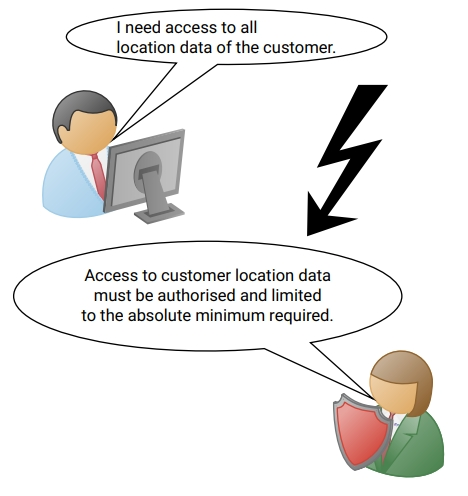
\includegraphics[width=0.35\textwidth]{Images/Prioritization und Negotiation.jpeg}
    \caption{Negotiation}
\end{figure}

\subsubsection*{Requirements Documentation}
\begin{defBox}[title=Documentation]
    The requirements are \red{documented} and used as \red{input} for the next iteration.\\
    The produced documents may be \red{formal} or \red{informal}.
\end{defBox}

\subsection{Requirements Documentation}
\subsubsection*{Software Requirements Specification Document (SRS)}

\begin{defBox}[title=Target group of SRS]
    Diverse set of stakeholders:
    \begin{itemize}
        \item Client, prospective users
        \item Managers (both on client and manufacturer side)
        \item System engineers, system test, and system maintenance engineers
        \item $\Rightarrow$ Anyone concerned with ordering, using, manufacturing, maintaining
    \end{itemize}
\end{defBox}
\begin{infoBox}
    Die Zielgruppe umfasst alle Personen, die in irgendeiner Weise mit dem \fatsf{Bestellen, Nutzen, Entwickeln oder Warten} der Software in Berührung kommen. Das SRS dient als gemeinsames Kommunikationsmittel, um sicherzustellen, dass alle Stakeholder die Anforderungen einheitlich verstehen.
\end{infoBox}
\begin{defBox}[title=Level of detail depends on ...]
    \begin{itemize}
        \item Type of system
        \item Development process
        \item Location of manufacture: external contractor or in-house
    \end{itemize}
\end{defBox}
\begin{infoBox}[title=Der Detaillierungsgrad des SRS hängt ab von ...]
    \begin{enumerate}
        \item \fatsf{Art des Systems}
        \begin{itemize}
            \item Ein komplexes System benötigt ein detailliertes SRS, während für kleinere, weniger komplexe Systeme ein einfacheres SRS ausreichen kann.
        \end{itemize}
        \item \fatsf{Entwicklungsprozess}
        \begin{itemize}
            \item In einem \fatsf{agilen Entwicklungsprozess} könnte das SRS eher allgemein sein und sich im Laufe der Zeit weiterentwickeln.
            \item In einem \fatsf{traditionellen Wasserfall-Modell} ist ein detailliertes und vollständiges SRS zu Beginn des Projekts erforderlich.
        \end{itemize}
        \item \fatsf{Ort der Fertigung: externer Auftragnehmer oder In-House\_Entwicklung}
        \begin{itemize}
            \item Wenn die Entwicklung durch einen \fatsf{externen Auftragnehmer} erfolgt, ist ein detailliertes SRS notwendig, um sicherzustellen, dass die Anforderungen klar und eindeutig sind.
            \item Bei einer \fatsf{In-House\_Entwicklung} kann das SRS flexibler sein, da die Entwickler näher am Projekt sind und schneller auf Änderungen reagieren können.
        \end{itemize}
    \end{enumerate}
\end{infoBox}

\subsection*{Structure of the Software Requirement Document}
\begin{defBox}[title=Requirements specification document (shortened from: ISO/IEC/IEEE 29148:2011)]
    \begin{enumerate}
        \item Introduction
        \begin{enumerate}
            \item Pupose of the requirements document (Zweck des Anforderungsdokuments)
            \begin{infoBox}
                Beschreibt, warum das Dokument erstellt wurde und welche Ziele es hat. Es legt fest, für wen das Dokument gedacht ist und welchen Nutzen es bietet.
            \end{infoBox}
            \item \blue{Scope of the product} (Umfang des Produkts)
            \begin{infoBox}
                Definiert, was das System leisten soll, also den \fatsf{Anwendungsbereich} des Produkts. Hier wird auch beschrieben, \fatsf{was nicht im Umfang enthalten} ist, um Messverständnisse zu vermeiden.
            \end{infoBox}
            \item Definitions, acronyms and abbreviations (Definitionen, Akronyme und Abkürzungen)
            \item References (Referenzen)
            \begin{infoBox}
                Eine Liste von \fatsf{Dokumenten, Standards} oder \fatsf{anderen Quellen}, auf die im Anforderungsdokument Bezug genommen wird.
            \end{infoBox}
            \item Overview (Überblick)
            \begin{infoBox}
                Eine \fatsf{kurze Zusammenfassung} des Dokuments, die beschreibt, wie es organisiert ist und welche Inhalte in den folgenden Abschnitten zu erwarten sind.
            \end{infoBox}
        \end{enumerate}
        \item General description
        \begin{enumerate}
            \item \blue{Product perspective}
            \begin{infoBox}
                Beschreibt, wie sich das System in \fatsf{andere Systeme} oder \fatsf{bestehende Produkte} einfügt, einschließlich seiner Schnittstellen und Abhängigkeiten.
            \end{infoBox}
            \item Product functions
            \begin{infoBox}
                Eine allgemeine Beschreibung der \fatsf{Hauptfunktionen}, die das System bereitstellen soll.
            \end{infoBox}
            \item \blue{User characteristics} (Benutzermerkmale)
            \begin{infoBox}
                Beschreibt die \fatsf{Zielgruppe} des Produkts, z.B. die \fatsf{Erfahrung} oder \fatsf{technischen Fähigkeiten} der Benutzer.
            \end{infoBox}
            \item Limitations (Einschränkungen)
            \begin{infoBox}
                Nennen von \fatsf{Einschränkungen} oder \fatsf{Bedingungen}, die bei der Entwicklung betrachtet werden müssen, z.B. rechtliche Anforderungen oder technische Grenzen.
            \end{infoBox}
            \item Assumptions and dependencies (Annahmen und Abhängikeiten)
            \begin{infoBox}
                \fatsf{Annahmen}, die während der Anforderungsanalyse gemacht wurden, und \fatsf{Abhängigkeiten}, die das System betreffen.
            \end{infoBox}
        \end{enumerate}
    \end{enumerate}
\end{defBox}
 \begin{defBox}
    \begin{enumerate}[start=3]
        \item Specific requirements (Spezifische Anforderungen)
        \begin{infoBox}
            Dieser Abschnitt enthält die detaillierten \fatsf{funktionalen} und \fatsf{nicht-funktionalen} Anforderungen. Es handelt sich um eine \fatsf{ausführliche Beschreibung} dessen, was das System leisten muss, und wie es sich unter bestimmten Bedingungen verhalten soll.
        \end{infoBox}
        \item Appendices, Index, etc. (Anhänge, Index usw.)
        \begin{infoBox}
            \begin{itemize}
                \item \fatsf{Anhänge} können zusätzliche Informationen enthalten, die für das Verständnis des Dokuments nützlich sind, z.B. \fatsf{Flussdiagramme, technische Spezifikationen} oder \fatsf{Beispiele.}
                \item Ein \fatsf{Index} hilft, bestimmte Abschnitte oder Begriffe im Dokument schnell zu finden.
            \end{itemize}
        \end{infoBox}
    \end{enumerate}
\end{defBox}
\begin{itemize}
    \item \red{1.b Scope of product:} Can also contain what is \red{not} in scope
    \begin{infoBox}
        Kann auch beschreiben, \fatsf{was nicht im Umfang enthalten} ist, um die Grenzen des Projekts klar fetzulegen.
    \end{infoBox}
    \item \red{1.c Glossary:} Explains ambiguous or technical terms, expand abbreviations
\end{itemize}

\subsection{Requirements Engineering Process}
\subsubsection*{Requirement Validation}
\begin{defBox}[title=Requirement Validation Checkpoints]
    \begin{itemize}
        \item \red{Validity} (Gültigkeit)
        \begin{itemize}
            \item Do the requirements \red{capture} the needed features?
            \item Is \red{additional} or other functionality needed?
        \end{itemize}
        \item \red{Consistency} (Konsistenz)
        \begin{itemize}
            \item Check that the requirements are \red{not conflicting}
        \end{itemize}
        \item \red{Completeness} (Vollständigkeit)
        \begin{itemize}
            \item Do the requirements define \red{all} functions and constraints as intended by the system user?
        \end{itemize}
        \item \red{Realism} (Realisierbarkeit)
        \begin{itemize}
            \item Can the requirements reasonably be implemented? (Refinement of feasibility study)
        \end{itemize}
        \item \red{Traceability} (Rückverfolgbarkeit)
        \begin{itemize}
            \item Is each requirement traceable to its source (where does each requirement derive from)?
            \begin{infoBox}
                \begin{itemize}
                    \item Jede Anforderung sollte auf ihren \fatsf{Ursprung} zurückgeführt werden können, d.h. es sollte klar sein, woher die Anforderung stammt (z.B. ein bestimmter Stakeholder, eine gesetzliche Vorschrift).
                    \item Die Rückverfolgbarkeit hilf dabei, \fatsf{Änderungen} an den Anforderungen nachzuvollziehen und sicherzustellen, dass alle Anforderungen korrekt abgedeckt sind.
                \end{itemize}
            \end{infoBox}
        \end{itemize}
    \end{itemize}
\end{defBox}